We address the problem of estimating disease comorbidity networks from longitudinal patient event sequences while adjusting for confounding by shared risk factors. To reach this goal, we model disease relationships using an undirected weighted graph $G=(V,E)$, where the node set $V$ represents diseases and the edge set $E$ encodes pairwise associations. Edge weights are stored in the weighted adjacency matrix $A$, whose entries $A_{ij}$ quantify the strength of the relationship between diseases $i$ and $j$ based on their co-occurrence and temporal ordering within patient trajectories. Our methodological pipeline, shown in Figure~\ref{fig:pipeline}, consists of six main stages, each addressing a key challenge in translating longitudinal patient data into interpretable disease networks. First in Section~\ref{subsection:seq_con}, we construct temporally ordered event sequences from patient histories to preserve chronological information that is lost in traditional prevalence-based approaches. Second in Section~\ref{subsection:word_embedding}, we learn dense vector representations of diseases and risk factors by adapting pretrained Word2Vec embeddings to longitudinal clinical data, enabling representations that capture both temporal context and biomedical semantics. Third, in Section~\ref{subsection:network_con} we construct dense disease similarity networks using cosine similarity between learned embeddings, yielding weighted networks that encode global semantic and temporal relationships among diseases. Fourth in Section~\ref{subsection:risk_factor}, we introduce a principled framework to evaluate and correct confounding induced by shared risk factors, enabling the derivation of adjusted disease similarity networks that better reflect direct pathophysiological relationships. Finally, in Sections~\ref{subsec:sparsification} and~\ref{subsec:topology}, we apply Gaussian Graphical Models with Lasso regularization to obtain sparse networks that capture conditional dependencies, facilitating interpretability, visualization, and topological analysis.

\begin{figure}[t]
    \centering
    \hspace*{-1.8cm}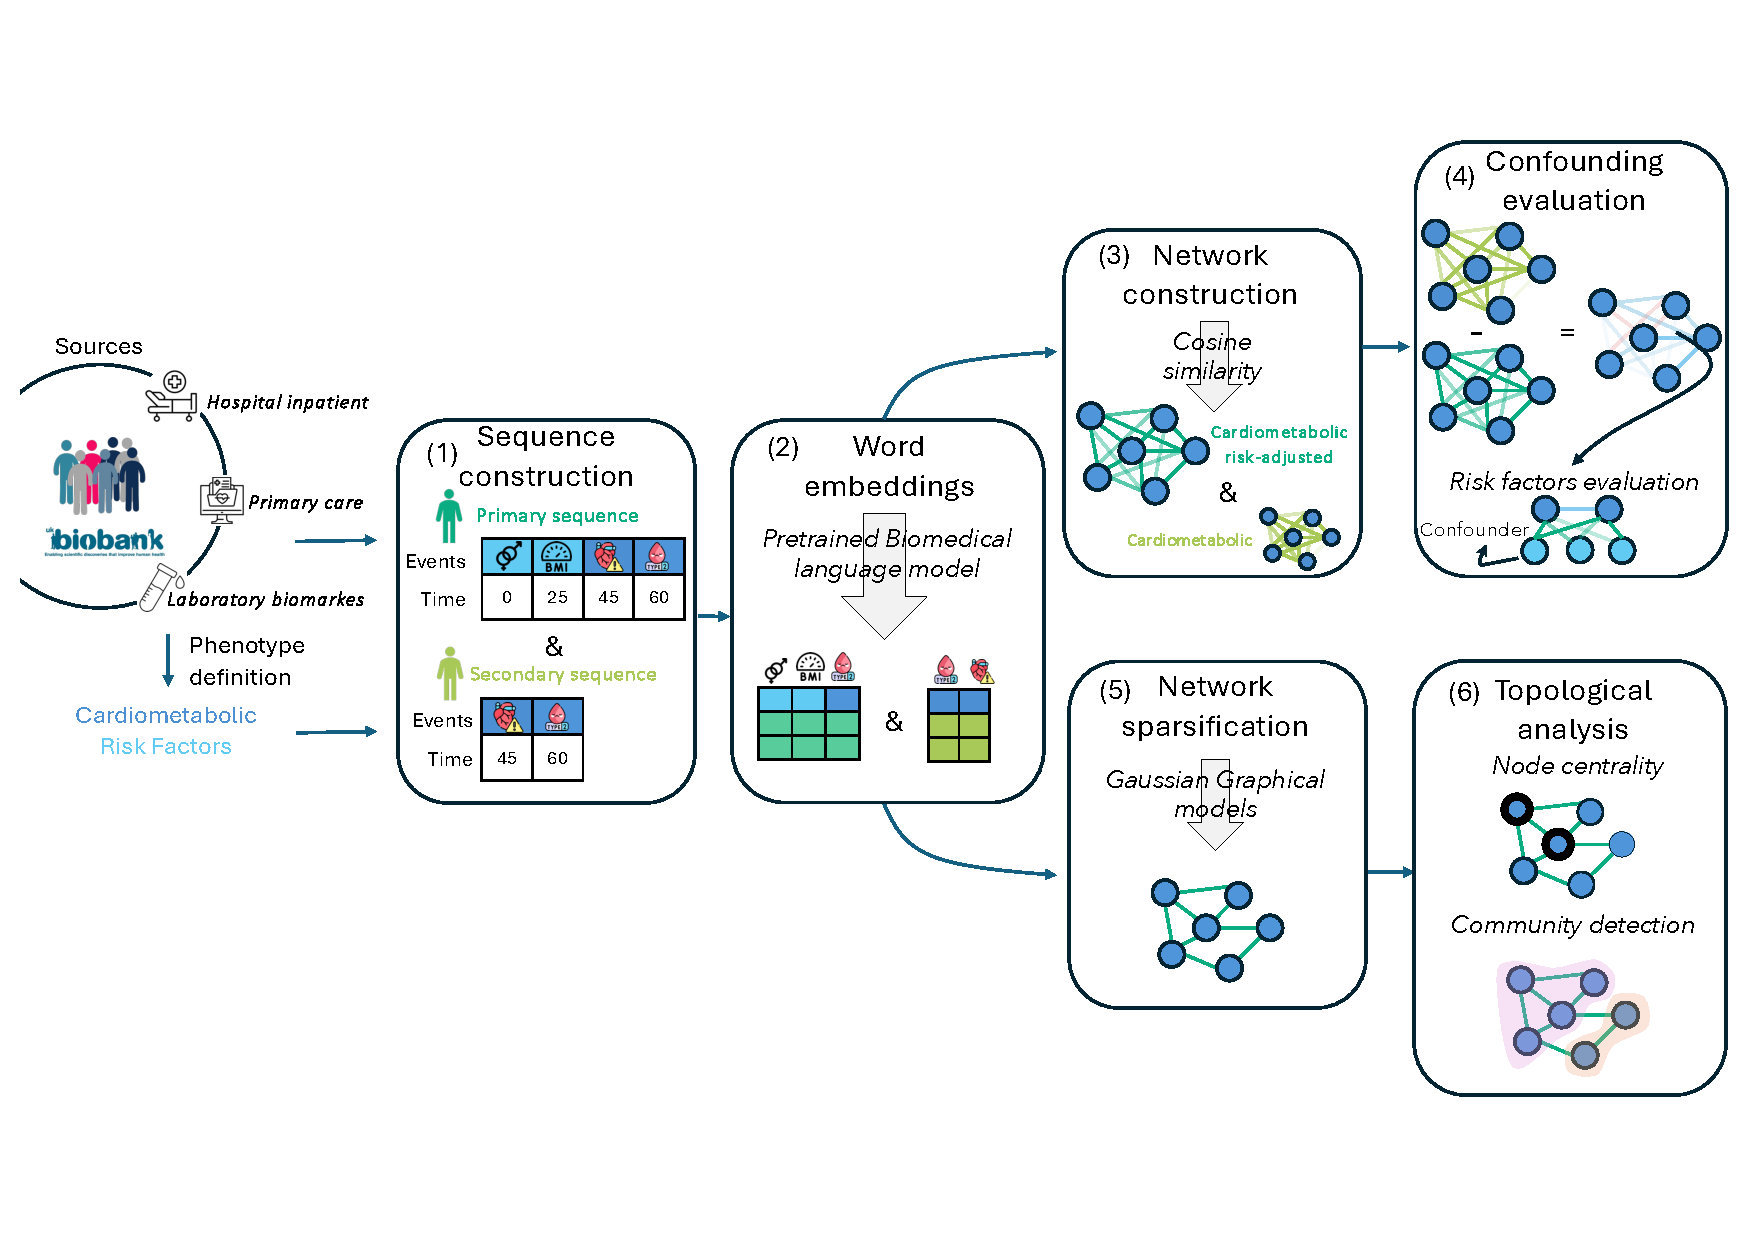
\includegraphics[width=1.3\linewidth]{Figures/pipeline.pdf}
    \caption{Schematic representation of the methodological framework for risk-adjusted cardiometabolic comorbidity network inference. The workflow proceeds through four primary stages: (1) Phenotype definition and sequence construction: integration of multimodal data sources, including hospital records, primary care data, and clinical biomarkers, to generate a primary sequence including both cardiometabolic diseases and risk factors and a secondary sequence restricted to cardiometabolic diseases. (2) Word embeddings: mapping of clinical events into a dense vector space by fine-tuning pretrained biomedical language models on cohort-specific patient sequences. (3-4) Network construction and confounding evaluation: estimation of pairwise cosine similarities to quantify disease associations and implementation of a systematic comparison between unadjusted and risk-adjusted networks to identify and remove confounding effects. (5-6) Network sparsification and topological analysis: sparse network construction via Gaussian Graphical Models to identify direct conditional dependencies, followed by the characterization of central disease hubs and the detection of disease modules through modularity optimization.}
    \label{fig:pipeline}
\end{figure}

\subsection{Sequence construction}\label{subsection:seq_con}
For each patient $p \in \{1, \ldots, P\}$, we construct a temporal event sequence:
\begin{equation}
S_p = \{(t_1, v_1), (t_2, v_2), \ldots, (t_{n_p}, v_{n_p})\},
\end{equation}
where $n_p$ denotes the number of recorded events, $v_j \in \mathcal{V}$ represents the event identifier (disease or risk factor), and $t_j \in \mathbb{R}_+$ denotes time from birth in days. Sequences are ordered chronologically such that $t_1 < t_2 < \cdots < t_{n_p}$. This temporal ordering enables the embedding model to capture both co-occurrence patterns and disease progression dynamics. We construct a primary sequence $S_p^{(\mathcal{D}+\mathcal{R})}$ containing events from the full vocabulary $\mathcal{V} = \mathcal{D} \cup \mathcal{R}$, where $\mathcal{D}$ denotes the set of cardiometabolic diseases and $\mathcal{R}$ the set of risk factors, yielding a vocabulary size $|\mathcal{V}^{(\mathcal{D}+\mathcal{R})}| = 122$. To evaluate the effect of risk factor adjustment, we also construct a secondary sequence $S_p^{(\mathcal{D})}$, restricted to cardiometabolic diseases, with vocabulary size $|\mathcal{V}^{(\mathcal{D})}| = D = 24$. In the following, we denote events $v_j \in \mathcal{D}$ by $d_j$ and events $v_j \in \mathcal{R}$ by $r_j$.

\subsection{Word embeddings}\label{subsection:word_embedding}
In natural language processing, representation learning maps words into a continuous, low-dimensional embedding vector space where geometric proximity reflects semantic similarity derived from contextual co-occurrence. We adapt the Word2Vec skip-gram architecture to longitudinal clinical data by conceptualizing medical events as ``words'' and entire patient trajectories as ``sentences''. The choice of this framework is motivated by the ability of Word2Vec to generate embeddings, in which entities appearing in similar clinical contexts, such as conditions with shared pathophysiological precursors, are mapped closely in the embedding space. This approach enables the efficient extraction of information from complex longitudinal sequences without increasing model complexity, effectively balancing representational power with computational efficiency. We leverage the pretrained BioWordVec model~\citet{zhang2019biowordvec}, which combines embeddings trained on 27 million PubMed abstracts with Medical Subject Headings (MeSH) structure, providing domain-specific biomedical knowledge. Each phenotype is tokenized into constituent words (e.g., ``Chronic Kidney Disease'' $\rightarrow$ [``Chronic'', ``Kidney'', ``Disease'']). We fine-tune BioWordVec on patient sequences using the original skip-gram configuration: embedding dimension $d=200$, context window size $c=5$, and standard learning rate schedule. To balance cohort-specific adaptation with preservation of biomedical semantics, we monitor the cosine similarity between pretrained and fine-tuned embeddings:
\begin{equation}
\text{sim}_{\text{preserved}}^{(t)} = \frac{1}{|\mathcal{V}|} \sum_{v \in \mathcal{V}} \frac{\mathbf{e}_v^{(t)} \cdot \mathbf{e}_v^{(0)}}{\|\mathbf{e}_v^{(t)}\| \|\mathbf{e}_v^{(0)}\|},
\end{equation}
where $\mathbf{e}_v^{(t)}$ denotes the embedding at epoch $t$ and $\mathbf{e}_v^{(0)}$ the pretrained embedding. Fine-tuning is stopped when $\text{sim}_{\text{preserved}}^{(t)} < 0.70$, ensuring at least $70\%$ semantic retention. In our application, this criterion was satisfied after 4 epochs. For phenotypes composed of multiple words (e.g., ``Chronic Kidney Disease"), let $W$ be the set of constituent tokens (e.g., $W \in \{\text{``Chronic"; ``Kidney"; ``Diseases"}\}$). The phenotype embedding is computed as the average:
\begin{equation}
\mathbf{e}_{\text{phenotype}} = \frac{1}{|\text{$W$}|} \sum_{w \in \text{$W$}} \mathbf{e}_w.
\end{equation}

\subsection{Network construction using cosine similarity}\label{subsection:network_con}
Following established practices in the literature~\citet{gundougan2020research}, to determine the relationship between phenotype embeddings and construct the weighted adjacency matrix $A$, we used pairwise cosine similarity. Given phenotype embeddings $\{\mathbf{e}_1, \ldots, \mathbf{e}_D\}$, the adjacency matrix $A \in [0,1]^{D \times D}$ is defined as:
\begin{equation}\label{eq:cosine_similarity}
A_{ij} = \text{sim}(\mathbf{e}_i, \mathbf{e}_j) = \frac{\mathbf{e}_i \cdot \mathbf{e}_j}{\|\mathbf{e}_i\| \|\mathbf{e}_j\|}.
\end{equation}
This produces a fully connected, weighted network where edge weights reflect overall semantic and contextual similarity between diseases. Cosine similarity ranges from $-1$ (opposite identical) to $+1$ (identical), with values near 0 indicating orthogonality in the embedding space (no shared meaning). We construct two disease similarity networks: $A^{(\mathcal{D}+\mathcal{R})}$, derived from embeddings learned from the primary sequences containing both cardiometabolic diseases and risk factors, and $A^{(\mathcal{D})}$, derived from embeddings trained on the secondary disease-only sequences.

\subsection{Confounding evaluation}\label{subsection:risk_factor}
\subsubsection{Conceptual framework}
We define confounding in the embedding space as follows: if diseases $d_i, d_j \in \mathcal{D}$ are associated in patient trajectories due to a share common risk factor $r_k \in \mathcal{R}$, then similarity computed from disease-only sequences, $A_{ij}^{(\mathcal{D})}$, is expected to be inflated related to the ``true" pathophysiological relationship. Jointly embedding diseases and risk factors redistributes part of this shared signal to the risk factor dimensions, yielding adjusted disease embeddings and corrected similarity estimates $A_{ij}^{(\mathcal{D}+\mathcal{R})}$.

\subsubsection{Statistical evaluation of changes}
We quantify similarity changes as:
\begin{equation}\label{eq:similarity_difference}
\Delta_{ij} = A_{ij}^{(\mathcal{D}+\mathcal{R})} - A_{ij}^{(\mathcal{D})}.
\end{equation}
Negative values ($\Delta_{ij} < 0$) indicate confounding removal (similarity decreased after adjustment), while positive values ($\Delta_{ij} > 0$) suggest unmasking of true relationships previously obscured by noise. We assess the global impact of risk adjustment using the Mean Absolute Difference (MAD) to quantify the average magnitude of change across all disease pairs and the Mean Directional Change (MDC) to assess systematic bias in adjustment direction: 
\begin{equation}
\text{MAD} = \frac{1}{D(D-1)/2} \sum_{i < j} |\Delta_{ij}|,\text{ } \text{ } \text{ } \text{MDC} = \frac{1}{D(D-1)/2} \sum_{i < j} \Delta_{ij},
\end{equation}
where negative MDC indicates systematic similarity decreases. We employed a Wilcoxon signed-rank test to test the null hypothesis $H_0: \text{median}(\Delta_{ij}) = 0$ against the alternative $H_1: \text{median}(\Delta_{ij}) \neq 0$, providing formal statistical evidence of systematic change. To evaluate preservation of network structure, we compute the Spearman rank correlation:
\begin{equation}
\rho_S = \text{corr}_{\text{Spearman}}(\{A_{ij}^{\mathcal{D}}\}_{i<j}, \{A_{ij}^{\mathcal{D+R}}\}_{i<j}),
\end{equation}
where a high correlation ($\rho_S \approx 1$) indicates structural preservation despite local adjustments.

\subsubsection{Confounding detection and validation}\label{subsub:conf_det}
To validate that observed similarity changes reflect genuine confounding removal rather than random noise, we implement a three-step analysis linking similarity changes to shared risk factors:

\textbf{Step 1: Identify highly affected pairs.} Disease pairs are ranked by $|\Delta_{ij}|$, and those in the 95-$th$ percentile of the distribution are selected.

\textbf{Step 2: Identify disease-risk factor associations.} For each disease $d_i \in \mathcal{D}$, associated risk factors $\mathcal{R}_i \subset \mathcal{R}$ are identified based on their embedding similarity. A risk factor $r \in \mathcal{R}$ is considered associated with disease $d_i \in \mathcal{D}$ if:
\begin{equation}\label{eq:rf_threshold}
\text{sim}(\mathbf{e}_{d_i}, \mathbf{e}_{r}) > \tau,
\end{equation}
where $\tau$ is the median pairwise similarity among all risk factors: 
\begin{equation} \tau = \text{median} \left( { \text{sim}(\mathbf{e}_{r_k}, \mathbf{e}_{r_l}) : 1 \le k < l \le R } \right). 
\end{equation}
This threshold ensures that only associations that are strong, relative to the global correlation structure induced by the risk factors' embedding, are further investigated.

\textbf{Step 3: Quantify shared risk factors.}
For disease pair $(d_i, d_j)$, the proportion of shared risk factors is computed as:
\begin{equation}\label{eq:shared_rf}
\text{SharedRF}_{ij} = \frac{|\mathcal{R}_i \cap \mathcal{R}_j|}{min(|\mathcal{R}_i|, | \mathcal{R}_j|)}.
\end{equation}
Under our confounding framework, high $|\Delta_{ij}|$ values are expected to correspond to large $\text{SharedRF}_{ij}$. To formally test this hypothesis, we use a Mann-Whitney U test to evaluate whether the distribution of $\text{SharedRF}_{ij}$ is stochastically greater in highly affected pairs (defined in Step 1) against that of all remaining pairs. A significant result would provide statistical evidence that confounding magnitude correlates with shared risk factor burden, validating our adjustment procedure.

Finally, to assess the robustness of the choice of the confounding detection threshold $\tau$, we repeat the analysis in a range of $\tau \in \{0.5, 0.6, 0.7, 0.8, 0.9\}$ and report for each threshold the proportion of shared risk factors in the highly affected pairs and the Mann-Whitney U test.

\subsection{Network sparsification using Gaussian Graphical Models}\label{subsec:sparsification}
Similarity-based networks are inherently fully connected, while this weighted adjacency matrix contains the complete set of pairwise relationships, the underlying structural properties are often obscured by the high edge density, complicating visualization, interpretation, and topological inference. Conventionally, sparsification is achieved by applying a global hard threshold, where edges are retained only if their weights exceed an arbitrary value. To move beyond such heuristic approaches, statistical "backboning" methods have been proposed to identify edges that are significantly stronger than a null model~\citet{foti2011nonparametric}. However, these methods typically assume a high degree of heterogeneity in the weight distribution and they fail to extract a meaningful latent geometry in fully connected networks where similarity values are relatively homogeneous or narrowly distributed. Consequently, to obtain a sparse and interpretable representation, we adopt a Gaussian Graphical Model (GGM) framework. Unlike cosine similarity, which captures overall contextual relatedness, a GGM estimates partial correlations that quantify the association between two diseases after conditioning on the influence of all other variables in the system. This approach provides a principled mechanism for direct sparsification through Lasso regularization, effectively pruning edges that do not represent direct conditional dependencies. A more detailed discussion on the limitations of traditional backboning methods in this context is provided in Supplementary Method~\ref{supp_met_1}.

Treating each embedding dimension as an independent observation~\citet{zhelezniak2019correlation}, the embedding vectors $\{\mathbf{e}_v\}_{v \in \mathcal{V}}$ are assumed to follow a multivariate Gaussian distribution $
\mathbf{e} \sim \mathcal{N}(\boldsymbol{\mu}, \boldsymbol{\Sigma})
$
where $\boldsymbol{\Sigma} \in \mathbb{R}^{(D+R) \times (D+R)}$ is the covariance matrix. Under this hypothesis, conditional independence is encoded in the precision matrix $\boldsymbol{\Omega} = \boldsymbol{\Sigma}^{-1}$ with $\omega_{ij} = 0$ if and only if embeddings $i$ and $j$ are conditionally independent given all other events. The multivariate normality assumption was evaluated using Shapiro-Wilk tests on each embedding dimension, with a significance threshold $\alpha = 0.05$. We employ a neighborhood selection approach~\citet{meinshausen2006high} to estimate $\boldsymbol{\Omega}$ through $D+R$ independent Lasso regression models. For each phenotype $i \in \mathcal{D \cup R}$, we solve:
\begin{equation}\label{eq:neighborhood_selection}
\hat{\boldsymbol{\beta}}^{(i)} = \mathop{\arg \min}_{\boldsymbol{\beta} \in \mathbb{R}^{R+D-1}} \|\mathbf{e}_i - \mathbf{E}_{-i}\boldsymbol{\beta}\|_2^2 + \lambda \|\boldsymbol{\beta}\|_1,
\end{equation}
where $\mathbf{E}_{-i}$ is the matrix of embeddings excluding phenotype $i$, and $\lambda > 0$ controls sparsity through the $\ell_1$ penalty. The estimated neighborhood of phenotype $i$ is:
\begin{equation}
\hat{E}_i = \{j : \hat{\beta}_j^{(i)} \neq 0 \text{ or } \hat{\beta}_i^{(j)} \neq 0\},
\end{equation}
using the OR rule to ensure symmetry. The binary adjacency matrix is then obtain as:
\begin{equation}\label{eq:ggm_adjacency}
A_{ij}^{\mathcal{(D+R)}} = \mathbb{I}(j \in \hat{E}_i).
\end{equation}
The regularization parameter $\lambda$ is selected via 10-fold cross-validation, minimizing mean squared prediction error.


\subsection{Network topology analysis}\label{subsec:topology}
To characterize the systemic importance of individual diseases and uncover the modular architecture of the cardiometabolic landscape, we performed a topological analysis on the sparse GGM-derived network. We quantified disease importance using two complementary centrality measures, each capturing a distinct aspect of clinical relevance within the comorbidity network. Degree centrality ($C_D$) assesses the local connectivity of a node by quantifying the number of its direct disease associations:
\begin{equation}
C_D(i) = \sum_{j=1}^D A_{ij}.
\end{equation}
Betweenness centrality ($C_B$) serves as a global measure of a node's influence by identifying diseases that bridge distinct pathophysiological domains:
\begin{equation}
C_B(i) = \sum_{s \neq i \neq t} \frac{\sigma_{st}(i)}{\sigma_{st}},
\end{equation}
where $\sigma_{st}$ denotes the total number of shortest paths between diseases $s$ and $t$, and $\sigma_{st}(i)$ is the subset of those paths passing through disease $i$. 

Finally, we identified cohesive disease modules by applying the fast greedy modularity optimization algorithm~\citet{clauset2004finding}. This approach partitions the network into communities by maximizing the modularity $Q$:
\begin{equation}
Q = \frac{1}{2m} \sum_{ij} \left(A_{ij} - \frac{C_D(i) C_D(j)}{2m}\right) \delta(c_i, c_j),
\end{equation}
where $m = \frac{1}{2}\sum_{ij} A_{ij}$ represents the total edge count, $c_i$ denotes the community assignment of node $i$, and $\delta(c_i, c_j) = 1$ if $c_i = c_j$ and 0 otherwise. The algorithm iteratively merges communities to maximize $Q$, producing a hierarchical dendrogram. We select the partition with maximum modularity as the final community structure.